\subsection{Autoencoder}

The autoencoder is a type of network used to learn efficient encodings of unlabeled data. 

Autoencoders are split into two parts. The encoder $E_\phi$ and the decoder $D_\theta$. The relationship between these can be articulated as such: 

\begin{figure}[h]
    \centering
    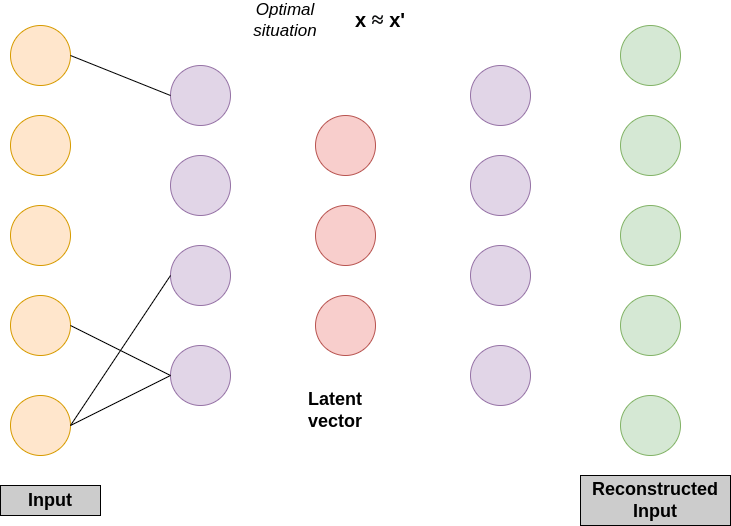
\includegraphics[scale=0.5]{figures/ae.png}
    \caption{Autoencoder Architecture Diagram}
    \label{fig:aediagram}
\end{figure}

\begin{equation}
E_\phi: X \rightarrow Z 
\end{equation}

\begin{equation}
D_\theta: Z \rightarrow X
\end{equation}

The optima for any kind of autoencoder becomes that of lossless encoding, which can further be described as such:

\begin{equation}
    X = D_\theta(E_\phi(X))
\end{equation}

When a auto encoder is trained to max effiency, we can in some cases remove the decoder part. Since the goal in the beginning was to map data to a lower-dimensional latent space, which has been increased. If ones goal is feature extraction, the decoder is not needed any more. Additionally, by removing the decoder, the overall complexity and size of the model $M$ decreases.


Typical usecases for autoencoders are signal analysis, anomaly detection, reconstructing images and so on. 
One of the more well known usages for autoencoders

\subsubsection{Variational Autoencoder (\acrshort{vae})}

Similar to the regular autoencoder, a \acrfull{vae} also aims to map input over to a feature representation. The diffre. Broadly speaking, the difference between a \acrshort{ae} and a \acrshort{vae} is that a AE maps input to points, where as VAEs map over to a distribution in the latent space. Thus, the \acrlong{vae} can be seemed as a generative model.


\begin{figure}[h]
    \centering
    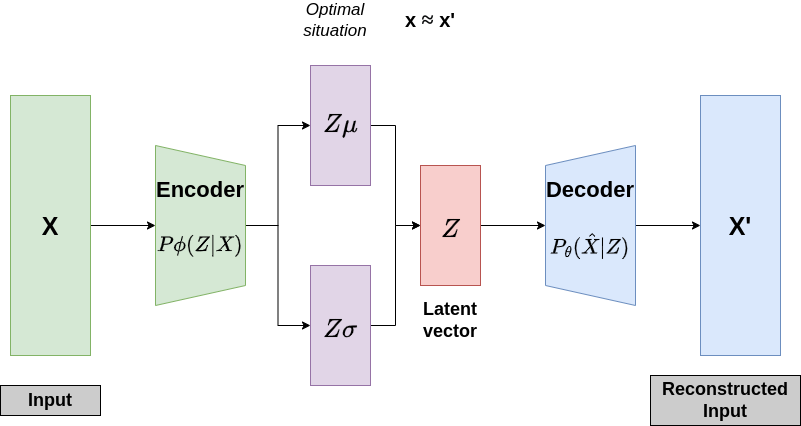
\includegraphics[scale=0.5]{figures/vae.png}
    \caption{Variational Autoencoder Architecture Diagram}
    \label{fig:vaediagram}
\end{figure}


VAEs can be trained by backpropagation due to something known as the \textit{reparametrization trick}. We need this because since VAEs maps to a stochastic variable, abckpropagation would else not be feasible.

\begin{align*}
\text{Given:} & \quad \text{Encoder LSTM outputs: } h \\
& \quad \text{Mean vector: } \mu \\
& \quad \text{Log variance vector: } \log(\sigma^2) \\
\text{Sample:} & \quad \epsilon \sim \mathcal{N}(0, 1) \\
\text{Reparameterization:} & \quad z = \mu + \sigma \odot \epsilon \\
\text{Decoder Input:} & \quad z \quad \text{(sampled latent vector)} \\
\text{Training Objective:} & \quad \text{Minimize reconstruction error} \\
& \quad \text{and KL divergence between } q(z|x) \text{ and } p(z) \\
\text{Loss Function:} & \quad \mathcal{L} = \text{reconstruction\_loss} + \text{KL\_divergence}
\end{align*}




\subsubsection{LSTM Variational Auto Encoder}

As we've discussed in \ref{ai:lstm} and \ref{ai:rnn}, these types of networks are well suited for . The issues found with \acrshort{rnn}s, such as long term dependencies, are solved with using \acrshort{lstm}s, and also initializing the weights in a more intelligent way. We are not going to make use of transfer learning for our network, thus we solely rely on \acrshort{lstm}s to solve these issues.

Combining the \acrshort{lstm} with an autoencoder approach, we'll be able to create a network well suited for anomaly detection on variable time series data.

\textbf{KEYS TO GETTING A GOOD VARIATIONAL AUTO ENCODER}

\begin{itemize}
    \item Pick the righ size for the latent space
    \item Learning rate scheduler  and hyperparam tuning 
    \item BETA COEFFICIENT
\end{itemize}

An effort has been made into trying to improve autoencoders for anomaly detection \cite{tan2023improving}

THIS ONE IS HIGHLY RELEVANT AND HAS MANY METRICS \cite{s23021009}